\documentclass{article}
\usepackage[utf8]{inputenc}


\usepackage{tikz}


\usetikzlibrary{shapes.geometric}
\usetikzlibrary{arrows.meta}
\usetikzlibrary{decorations.pathreplacing}
\newcommand*{\tikzgrid}[2]{\draw[help lines](0,0)grid[step=0.2,lightgray,ultra thin](#1,#2);\draw[help lines](0,0)grid[gray](#1,#2);\foreach\x in{0,1,...,#1}\node[below]at(\x,0){\scriptsize\x};\foreach\y in{1,2,...,#2}\node[left]at(0,\y){\scriptsize\y};}

\setlength{\unitlength}{20pt}

\usepackage{pict2e}
\usepackage{graphpap}

\begin{document}
	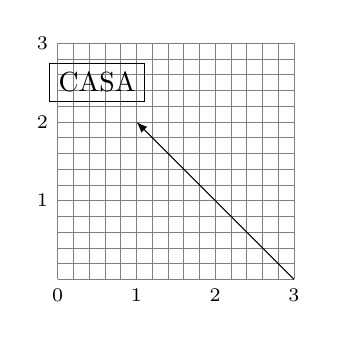
\begin{tikzpicture}
	\tikzgrid{3}{3}
	\draw[->,>=latex](3,0)--(1,2);
	\node[draw] at(0.5,2.5){CASA};
	\end{tikzpicture}
	\newpage
\begin{figure}
	\begin{center}
	\begin{picture}(25,15)
		\put(5.3,9.9){$x_1$}
		\put(0.835,14.2){$x_2$}
		\put(20.3,9.9){$y_1$}
		\put(15.77,14.2){$y_2$}
		\put(0.835,4.5){A}
		\put(15.77,4.5){$J_{A}$}
		%\multiput(2,2)(1,1){5}{$\int$}
		\qbezier(1,5)(1,10)(1,13.9) %x_2
		\qbezier(-3,10)(1,10)(5,10) %x_1
		\qbezier(16,5)(16,10)(16,13.9)%y_2
		\qbezier(12,10)(16,10)(20,10)%y_1
		\qbezier(-2.5,10.5)(0,11.1)(0.5,13.5)%first curva
		\qbezier(19.5,10.5)(17,11.1)(16.5,13.5)%second curva
		\qbezier(6,11)(8.5,14)(11,11)%primer curva vector
		\put(8.5,12.5){\vector(1,0){0.2}}
		\put(8.3,13){$L_p$}
		\qbezier(6,9)(8.5,6)(11,9)
		\put(8.5,7.5){\vector(-1,0){0.2}}
		\put(8.3,6.6){$L_p^{-1}$}
		\put(-4,12){$\varphi_{x_0}=L_p^{-1}.\varphi_{y_0}$}
		\put(17.5,12){$y_0=P_{x_0}$}
		\thinlines
		\thicklines
		\linethickness{10cm}
%		\graphpaper[1](0,0)(20,15)
		\put (0,12.16){\circle*{0.15}}
		\put (17.12,12){\circle*{0.15}}
		\put (0.2,11.8){$x_0$}
		\put (19.55,10.67){$\varphi_{y_0}$}
		
%		\line(4,3){1pt}
%		\vector(x0,y0){longitud}
%		\circle{diámetro}
%		\circle*{diámetro}
%		\oval(x,y)[parte]
%		\shortstack{columna}
%		\qbezier[num](x1,y1)(x2,y2)(x3,y3)
	\end{picture}
	\caption{}
	\end{center}
\end{figure}
\end{document}
